\section{Driver}\label{sec:driver}
\todo[color=c05b,inline]{testing the colors}

To control the MOSFETs the Semikron SKYPER 32 R driver board has been chosen.
It can run two MOSFETs or IGBTs potential free with up to 1200V over the device.
It supports an output of 15V PWM with peak currents to 15A at frequencies up to 50kHz.
The board also comes with additional protection logic that was not used as failure detection and shut down input.
The input to the board are two PWM signals coming from the controller with Voltages of 0 to 15V.
To function the SKYPER board needs an external power supply of 15V,
some decoupling capacitors and capacitors to filter high frequency pulses.
These components are on the adaptor board also from Semikron.

%%\begin{figure}[ht]
%%	\centering
%%	\includegraphics[width=1\textwidth]{figures/05mathematicalModelling/flowVsPowerRun34.eps}
%%	\caption{Data Points for Flow vs. Power Consumption}
%%	\label{fig:flowVsPowerConsumption}
%%\end{figure}

On the secondary side of the board the two potential free PWM signals with -8 to 15V are given out.
To adjust the switching properties of the device the output can be configured by changing the resistors Ron and Roff.
They limit the current when switching in the state, so the device will switch slower.
Additionally external decoupling capacitors are needed. They are also on the adaptor board.
The failure detection logic was not used for testing.

\begin{figure}[H]
   \centering
   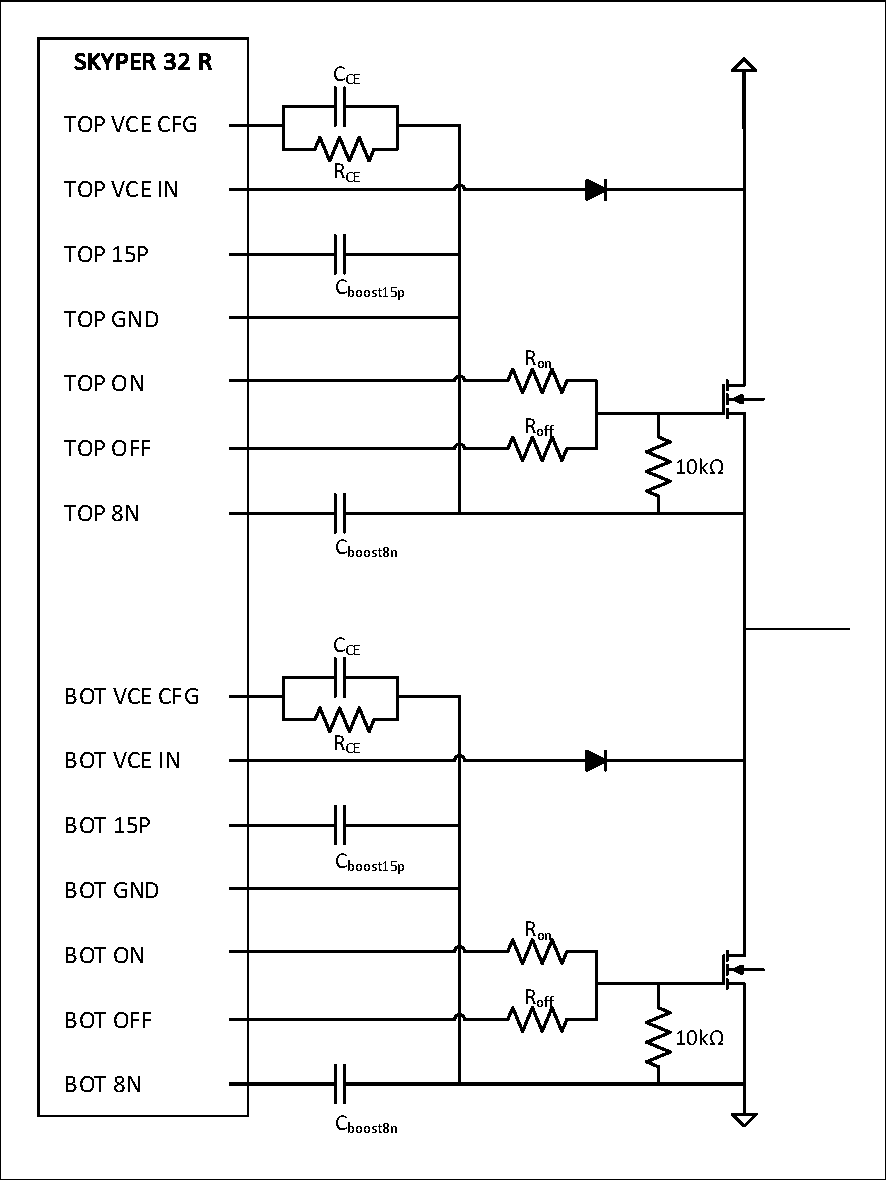
\includegraphics[width=\textwidth]{figures/Skyperboard/Skyper32out.pdf}
    \caption{Circuit on the output of the SKYPER 32R}
	\label{fig:ConventionalBoostONN}
\end{figure}


As the SKYPER Board needs an input signal of 15V a circuit is needed to convert the 5V signal from the low power logic.
Therefore a small comparator circuit was constructed.
It compares the input signal to XXX Volts, so every input above will result in a high output,
all inputs below as low.
This also allows to run it from a logic that only outputs 3V signals.